% ============================================================
% CHI 2027 Paper -- Initial Anonymous Submission
% ACM Primary Article Template (current: acmart v2.19)
%
% CHI 2027 review format:
%   single-column + line numbers + anonymous authors
%
% IMPORTANT:
%   This .tex file is compatible with the current CHI 2027 format,
%   but the actual template version is determined by acmart.cls.
%   If kpsewhich/grep reports acmart v2.03, LaTeX is still compiling
%   with v2.03 until the class/package is updated.
%
% After conditional acceptance, change ONLY the class options to:
%   \documentclass[sigconf]{acmart}
% ============================================================

\documentclass[manuscript,review,anonymous]{acmart}

% ------------------------------------------------------------
% Packages
% Keep the preamble minimal for ACM/TAPS compatibility.
% acmart already loads many common packages.
% ------------------------------------------------------------
\usepackage{graphicx}
\usepackage{booktabs}
\usepackage{multirow}

% Older/minimal TeX installations may not include acmart's preferred
% Libertine fonts.  Use the scalable Latin Modern fallback in that case;
% otherwise microtype's font expansion fails on bitmap Computer Modern.
\IfFileExists{libertine.sty}{}{\usepackage{lmodern}}

\graphicspath{{figures/}}

% ------------------------------------------------------------
% BibTeX logo (as in ACM templates)
% ------------------------------------------------------------
\AtBeginDocument{%
  \providecommand\BibTeX{{Bib\TeX}}%
}

\begin{document}

% ============================================================
% Title
% ============================================================
\title{From Script to Performance: Context-Aware and Editable LLM Assistance for Conversational Character Animation}

% Keep the review source itself anonymized as well.
\author{Anonymous Author(s)}

% ============================================================
% Abstract
% ============================================================
\begin{abstract}
AI-assisted animation systems increasingly support generation and low-level refinement, yet conversational character performance also depends on interpretive decisions about what each character is doing, attending to, and expressing over time. We present a context-aware authoring workflow that exposes these decisions as editable \textit{Semantic Performance Tags} between narrative interpretation and animation execution. For dyadic dialogue, a pretrained large language model proposes an initial performance state for both characters and sparse dialogue-anchored semantic beats; the Maya interface projects the resulting canonical plan into two character-specific tag panels where animators can inspect and revise acting-related affect, attention, head, and blink decisions before deterministic compilation to JALI and Maya controls. The representation supports revising one or multiple semantic decisions across either character while keeping the dialogue immutable and avoiding an additional LLM call for tag edits. We evaluate the approach in two complementary studies: a within-subject authoring study comparing Direct Generation with Editable Semantic Performance Tags, and a text-only context ablation examining how additional conversational context affects proposed performance decisions. Results show \textbf{[headline Study~A / RQ2--RQ3 result]}, while the context ablation finds \textbf{[headline Study~B / RQ1 result]}. These findings suggest \textbf{[replace with a results-supported implication after analysis]}.

\end{abstract}

% ============================================================
% CCS Concepts
% Replace/refine these using the ACM CCS tool before submission.
% ============================================================
\ccsdesc[500]{Human-centered computing~Interactive systems and tools}
\ccsdesc[300]{Computing methodologies~Animation}
\ccsdesc[300]{Computing methodologies~Natural language processing}

% ============================================================
% Keywords
% ============================================================
\keywords{character animation, animation authoring, large language models,
expressive animation, human-AI interaction, creative tools}

\maketitle

% ============================================================
% Main paper
% Section numbering is generated automatically by LaTeX.
% ============================================================

\section{Introduction}

Character performance is shaped by more than the words a character speaks. In conversational animation, an animator may consider who is speaking, who is being addressed, what has occurred earlier in the scene, the relationship between characters, and what a character may be attempting to communicate or conceal. These contextual interpretations influence performance choices such as when a character establishes or avoids eye contact, how strongly the head participates in a gaze shift, whether an expression is sustained or suppressed, and how a character reacts while listening. A short utterance such as \emph{“I’m fine,”} for example, may support substantially different performances depending on whether it follows a casual question, an accusation, or an emotionally significant event. Authoring such performances therefore involves not only producing facial motion, but interpreting narrative and interpersonal context and translating that interpretation into temporally coordinated animation decisions.

Procedural and data-driven animation systems have substantially reduced the effort required to produce lower-level character motion. Systems such as JALI generate expressive, editable speech animation from audio and transcripts, while subsequent approaches such as VisemeNet produce animator-centric speech motion curves directly from audio \cite{edwards2016jali,zhou2018visemenet}. More recently, large language models (LLMs) have enabled natural-language interfaces for animation generation and control. Huang et al. demonstrated that LLM-generated structured commands can drive rigged characters \cite{huang2023realtime}; Keyframer combines natural-language generation with animation variants and direct editing \cite{tseng2025keyframer}; and LogoMotion provides code-connected editing widgets for modifying generated motion, grouping, and timing \cite{liu2025logomotion}. These systems demonstrate that LLMs can lower barriers to animation generation while still supporting iterative human refinement.

Recent work has also begun to connect textual context to character facial behavior. Prompt-to-Animation, for example, uses LLMs to map narrative scenarios grounded in the OCC emotion model to FACS Action Units and demonstrates that the resulting expressions can communicate contextual affect without custom model training \cite{durupinar2025prompt}. This suggests that contemporary LLMs can provide a useful source of high-level interpretation in addition to low-level animation control. However, generating an appropriate facial expression from narrative context does not by itself address how an animator authors a performance when multiple interpretations are plausible.

The limitation we address is therefore not that existing AI animation systems are uneditable. Both Keyframer and LogoMotion show the value of combining generation with direct manipulation and localized editing \cite{tseng2025keyframer,liu2025logomotion}. Rather, the object being edited is typically the generated animation, code, or motion parameters. For character acting, an undesirable motion may instead originate from a higher-level disagreement: the system may have inferred the wrong communicative intent, selected the wrong social target, interpreted avoidance as engagement, or assigned an inappropriate relationship between expression and gaze. When this interpretive layer remains implicit, an animator must infer why the system produced a behavior before deciding how to revise it. Editing a gaze trajectory, for example, is different from communicating that the character should avoid eye contact because they are concealing information.

Work on human-AI creative tools provides evidence that exposing intermediate abstractions can support more meaningful intervention. DreamGarden externalizes an LLM-generated hierarchical plan and allows users to modify an otherwise semi-autonomous generation process through operations such as pruning, extending, and providing feedback \cite{earle2025dreamgarden}. Piet similarly demonstrates the value of designing domain-specific interactive representations around the progressive workflows of creative professionals \cite{shi2024piet}. These systems motivate our central question: \textbf{what should an intermediate representation look like when the object being authored is not an implementation plan or a visual parameter, but a character's interpretation and performance within a conversation?}

We explore this question through a context-aware LLM-assisted authoring workflow for conversational character animation. Our approach introduces an intermediate \textbf{Performance Plan} between narrative interpretation and animation execution. We focus on authoring the performance of a target character in a dyadic conversation, while using information from both participants in the interaction. The system considers structured context including dialogue turns, speaker and addressee information, preceding conversational context, character relationships, and the current utterance. From this context, the LLM proposes semantic performance events describing dimensions such as communicative intent, affect, gaze target and timing, gaze avoidance and re-engagement, head involvement, and related facial-performance parameters. Each event can additionally contain a concise, user-facing rationale linked to observable dialogue or scene evidence.

Crucially, the Performance Plan is not treated as a hidden intermediate step on the way to a generated animation. It is presented to the animator as an editable authoring representation. Our interface allows animators to inspect performance decisions alongside dialogue and timeline context, modify individual semantic parameters, preserve or lock satisfactory decisions, and selectively regenerate others. The resulting plan is then translated into procedural facial-animation controls and executed through JALI within Maya. In this workflow, the LLM does not determine a final performance autonomously. Instead, it proposes an interpretation that can be accepted, contested, or revised before being committed to low-level animation.

We investigate this approach through three research questions:

\textbf{RQ1:} How does conversational and narrative context affect the appropriateness of LLM-proposed character performance decisions?

\textbf{RQ2:} How does an editable semantic Performance Plan affect animators' perceived control and their ability to iteratively refine AI-assisted character animation?

\textbf{RQ3:} How do animators accept, modify, reject, and reinterpret AI-generated performance suggestions during the authoring process?

To investigate these questions, we develop a prototype integrating context-aware performance interpretation, an editable Performance Plan, and procedural character-animation generation. We evaluate the system in a within-subject study with \textbf{[N] participants with character-animation experience}, comparing \textbf{[baseline condition]} with the proposed Performance Plan workflow across \textbf{[N] conversational scenes}. We examine authoring behavior including completion time, localized edits, regeneration patterns, and the acceptance, modification, or rejection of AI suggestions, together with perceived control, workload, and qualitative accounts of how participants incorporated or contested AI interpretations. \textbf{[Replace with final study design and headline results after data collection.]}

This work makes three contributions. First, we introduce a domain-specific intermediate representation that externalizes LLM interpretations of conversational character performance as inspectable and editable semantic decisions. Second, we present a mixed-initiative authoring workflow that connects narrative context to procedural facial-animation controls while supporting localized modification, preservation, and regeneration of performance choices. Third, through an empirical study with animators, we characterize how human creators accept, revise, and contest AI-generated performance interpretations, and derive implications for designing human-AI creative tools in domains where generation depends on subjective interpretation rather than a single correct output.

\section{Related Work}

Related work will be discussed here.
\section{Designing for Editable Performance Interpretation}

\subsection{Formative Interviews}

We conducted semi-structured interviews with five practitioners involved in authoring or directing character performance. Four participants had professional experience in animation or CG production, including film animation, game cinematics, previs, and 3D game animation, while one participant was a senior game designer. Participants were 26--33 years old and reported between 2 and 10 years of relevant professional experience. We intentionally included both animation and game-production perspectives because the proposed workflow concerns not only low-level facial-animation execution but also upstream decisions about character intent and performance direction. Table~\ref{tab:formative-participants} summarizes their backgrounds.

\begin{table}[t]
    \centering
    \caption{Backgrounds of formative-interview participants.}
    \label{tab:formative-participants}
    \begin{tabular}{lll}
        \toprule
        \textbf{ID} & \textbf{Primary background} & \textbf{Experience} \\
        \midrule
        P1 & Film animator & 10 years \\
        P2 & Game cinematic animator/director & 4 years \\
        P3 & CG short-film director / previs / animation & 6 years \\
        P4 & Senior game designer & 2 years \\
        P5 & 3D game animator & 3.5 years \\
        \bottomrule
    \end{tabular}
\end{table}

Participants were recruited through email and professional or social-media networks. Interviews were conducted remotely in English and lasted approximately one hour. Participants received no monetary compensation. All participants provided informed consent, and the study was conducted under the authors' institutional ethics approval. Interview records were transcribed and anonymized for analysis.

The interview proceeded in two parts. The first part used open-ended questions to examine participants' existing performance-authoring practices, including how they interpret dialogue and make decisions about gaze, facial expression, head motion, and blinking. We also discussed their prior experience with speech-driven facial animation and where such automation becomes insufficient for character performance.

Before discussing AI-assisted editing, participants who were not familiar with the relevant type of speech-driven or JALI-based facial animation were shown a short example to establish a shared understanding of the type of animation considered in this work. Participants who were already familiar with comparable workflows were not shown this example. The example was used only for orientation rather than as a common evaluation stimulus.

The later part of the interview introduced several interaction concepts as design probes, including structured semantic performance decisions, selective preservation and regeneration, and brief rationales for AI-generated behaviors. These concepts were introduced only after the discussion of participants' existing practices. This ordering allowed us to distinguish recurrent workflow concerns from participants' reactions to proposed interaction mechanisms.

We analyzed the interview data using reflexive thematic analysis \cite{braun2006thematic,braun2019reflexive}. OpenAI ChatGPT was used to assist the initial organization of recurring concepts and candidate codes across the interview transcripts. The first author subsequently reviewed these codes against the complete interview records, revised or merged them where necessary, and verified the interpretation of all excerpts reported in the paper. The reviewed codes were then iteratively organized into higher-level themes. We retained divergent responses rather than requiring agreement across participants.

\subsection{Findings}

\paragraph{Performance begins with an acting direction, but is judged through the resulting image.}

Across participants, performance authoring was described as beginning above the level of animation curves. Participants first considered character motivation, personality, emotional state, relationships, preceding events, and subtext before deciding how a character should behave. P1 described direct manipulation without an acting direction as difficult because there was no clear performance target, while P4 similarly emphasized establishing what the character is trying to do before specifying individual behaviors.

Participants did not, however, uniformly prefer a textual semantic representation over generated animation. P2 and P4 preferred seeing the system's interpretation before committing to animation, whereas P3 and P5 considered the visual result more immediate for judging whether an acting choice worked. P3 also noted that key poses could communicate performance more directly than textual descriptions. P5 preferred seeing animation first while still finding structured semantic descriptions useful for understanding and revising it. Semantic representation therefore appeared most useful when coupled with visual evaluation rather than used as its replacement.

\paragraph{Performance choices depend on narrative context, but also on production context.}

Participants consistently described facial performance as context dependent. Character personality, internal state, relationships, prior dialogue, and the current dramatic purpose influenced decisions about expression and gaze. Gaze in particular was described as intentional rather than arbitrary: participants associated eye contact, gaze avoidance, and re-engagement with attention, attitude, thought, emotional withdrawal, and the progression of a scene.

Participants also emphasized factors beyond narrative semantics. Shot scale, camera direction, staging, performance rhythm, and available rig controls could alter how a facial performance should be realized. Close-ups, for example, motivated finer eye and blink design, whereas broader or highly dynamic shots reduced the importance of subtle facial behavior. These observations reveal a broader production context than the current prototype attempts to model.

\paragraph{Useful automation requires preservation, but facial behaviors cannot always be edited independently.}

Participants generally viewed generated facial animation as a starting point rather than a final result. Several valued the ability to retain satisfactory parts of a generated performance while revising only what remained incorrect. P2 and P4 were especially explicit about preserving accepted output rather than regenerating the entire performance whenever one aspect was unsatisfactory.

At the same time, selective editing was not understood as complete independence between facial channels. P3 emphasized that gaze, expression, head motion, and other aspects of performance are perceptually coupled: changing one behavior may require corresponding changes elsewhere to maintain coherence. Participants were more consistently comfortable preserving high-level decisions or adjusting global properties such as strength than freezing every low-level channel independently.

\paragraph{Explanations are useful when interpretation is uncertain, but should not interrupt authoring.}

Participants expressed mixed interest in explanations of AI behavior. Some valued knowing why the system proposed an unexpected acting choice, particularly when a concise explanation helped them determine whether the system had interpreted the scene as intended. P4 considered the reasoning behind an acting choice especially useful, with supporting context available when more detail was needed.

Others placed substantially less value on explanations. P3 preferred quickly correcting an incorrect performance during production rather than reading its rationale, while P5 wanted only enough information to understand the system's intention before modifying the result. Participants also warned that verbose explanations or attempts to justify an obviously inappropriate result could interrupt the creative process.

\subsection{Design Goals}

Taken together, the findings motivated four design goals. These goals synthesize both recurrent workflow concerns from the open-ended portion of the interviews and participants' reactions to the later design probes, rather than treating each probe response as a direct feature requirement.

\textbf{DG1 --- Couple semantic performance decisions with visual feedback.}
The system should expose animator-meaningful performance concepts while allowing users to evaluate their realization in animation. The Semantic Performance Tag representation therefore functions alongside, rather than instead of, the Maya preview.

\textbf{DG2 --- Represent narrative and interpersonal state across both interlocutors.}
The system should preserve character identity, speaker/listener structure, preceding dialogue, relationships, and relevant scene information when proposing performance. Because a conversational beat may be driven by what one character says and what the other hears, speaking and listening behavior should be interpreted within one shared conversational context rather than as two unrelated target-character problems. Shot composition and rig-specific constraints remain outside the current semantic model and are handled through visual preview and subsequent Maya refinement. For gaze, this separation is explicit: the semantic representation specifies the semantic attention target---who or what the character attends to---while the animator calibrates its shot-specific visual realization in Maya. The same semantic target can therefore be realized differently across camera viewpoints without changing the underlying acting decision.

\textbf{DG3 --- Support local but coordinated revision.}
Users should be able to revise a disputed acting or attention decision without replacing the complete performance. Revision should occur at the semantic level---for example, changing an affect, persistent attention target, or temporary check---while deterministic execution remains responsible for translating the edited state into coordinated animation controls.

\textbf{DG4 --- Keep interpretation lightweight and available during authoring.}
The interface should expose a concise natural-language acting interpretation for the initial state and each meaningful beat, so that animators can understand the intended performance without reading a verbose explanation for every low-level behavior. These descriptions communicate the proposed acting choice rather than hidden model reasoning or chain-of-thought.

\subsection{Interaction Scope and Semantic Performance Tags}

These design goals motivated an authoring representation that sits between narrative interpretation and low-level facial animation. We focus on dyadic conversational authoring. Both interlocutors are represented within one shared semantic proposal; the system does not generate two independent target-character outputs and merge them afterward. Internally, the backend stores this proposal as a canonical Performance Plan. For authoring, Maya projects the same content as two character-specific \textit{Semantic Performance Tag} panels over one immutable dialogue. The underlying proposal contains an initial performance state for both characters followed by sparse semantic beats anchored to that dialogue.

The initial state specifies, for each character, an open-language acting interpretation, a visible affect state with intensity, a persistent attention target, and an optional persistent head state. A semantic beat records a meaningful executable change for one actor at a dialogue-word anchor. Each emitted beat contains a concise acting interpretation together with at least one changed executable channel---affect, attention, head, or blink. Acting-only interpretations are omitted because they do not correspond to an authorable executable change in the current prototype. When several semantic channels change at the same meaningful moment for the same actor, they are represented within the same beat rather than split into redundant events. Because the proposal is conversation-level, a listener beat may be anchored to the earliest semantically sufficient cue in another character's utterance rather than waiting for a turn boundary.

At the semantic level, attention distinguishes persistent focus from a brief check. Persistent focus remains active until a later attention change, whereas a brief check temporarily redirects gaze before returning to the prior persistent target. Targets may be either interlocutor, a non-animated person, a physical object or location, or one of a small set of directional aversions. Directional choices are used as context-dependent acting priors for internal attention or social avoidance rather than fixed psychological codes. Geometric look-at coordinates are not part of the Semantic Performance Tag representation and are resolved only during deterministic execution. This separation is deliberate: a semantic target such as the interlocutor remains stable across shots, while its visual realization may need to change with camera angle, staging, and character rig. The animator can therefore preserve the intended attention relationship while calibrating a gaze pose that remains visually readable in the current shot.

Visible affect uses a closed executable vocabulary corresponding to supported JALI states, with an explicit intensity, whereas the acting interpretation remains open natural language. This separation lets the model describe a nuanced acting idea without requiring every description to map one-to-one onto an executable facial label. Head and blink are optional supporting channels rather than mandatory components of every beat.

\begin{table}[t]
    \centering
    \caption{Semantic information exposed through the shared dyadic Semantic Performance Tag representation.}
    \label{tab:semantic-performance-tags}
    \begin{tabular}{p{0.20\columnwidth} p{0.30\columnwidth} p{0.40\columnwidth}}
        \toprule
        \textbf{Unit} & \textbf{Fields} & \textbf{Role} \\
        \midrule
        Initial dyadic state &
        per-character acting, affect, attention, optional head &
        Establishes the starting interpretation and persistent attention for both interlocutors. \\

        Semantic beat &
        actor, dialogue-word anchor, acting &
        Marks a meaningful character-specific change while retaining a shared conversational context. \\

        Affect change &
        state, intensity &
        Changes the visible executable affect only when the performance meaningfully shifts. \\

        Attention change &
        persistent focus or brief check, semantic target &
        Represents persistent social attention, temporary checks, object/person attention, or directional aversion. \\

        Supporting behavior &
        optional head, blink &
        Adds executable supporting behavior when required by the acting beat. \\
        \bottomrule
    \end{tabular}
\end{table}

The Semantic Performance Tag representation is intentionally sparse: the absence of a channel in a beat means that the corresponding semantic state does not change. It is not intended to replace visual authoring or to imply that facial behaviors are perceptually independent. Instead, it provides a semantic surface for identifying \textit{what} the animator wishes to change while leaving temporal realization, rig coordinates, and curve generation to the deterministic execution layer. This separation allows the LLM to propose a shared conversational interpretation, the animator to revise that interpretation at an authorable semantic level, and JALI and Maya to realize the current edited semantic proposal as animation.

\section{System}

We implemented a Maya-based prototype that separates conversational performance interpretation from animation execution. The participant-facing tool runs in Autodesk Maya 2025 using PySide6, while LLM generation and canonical-plan compilation run in a separate Python backend. The backend stores a validated sparse \textit{Performance Plan}; Maya projects it as two character-specific \textit{Semantic Performance Tag} editors over the same dialogue. After generation, editing and execution are deterministic (Figure~\ref{fig:system-overview}).

\begin{figure*}[t]
    \centering
    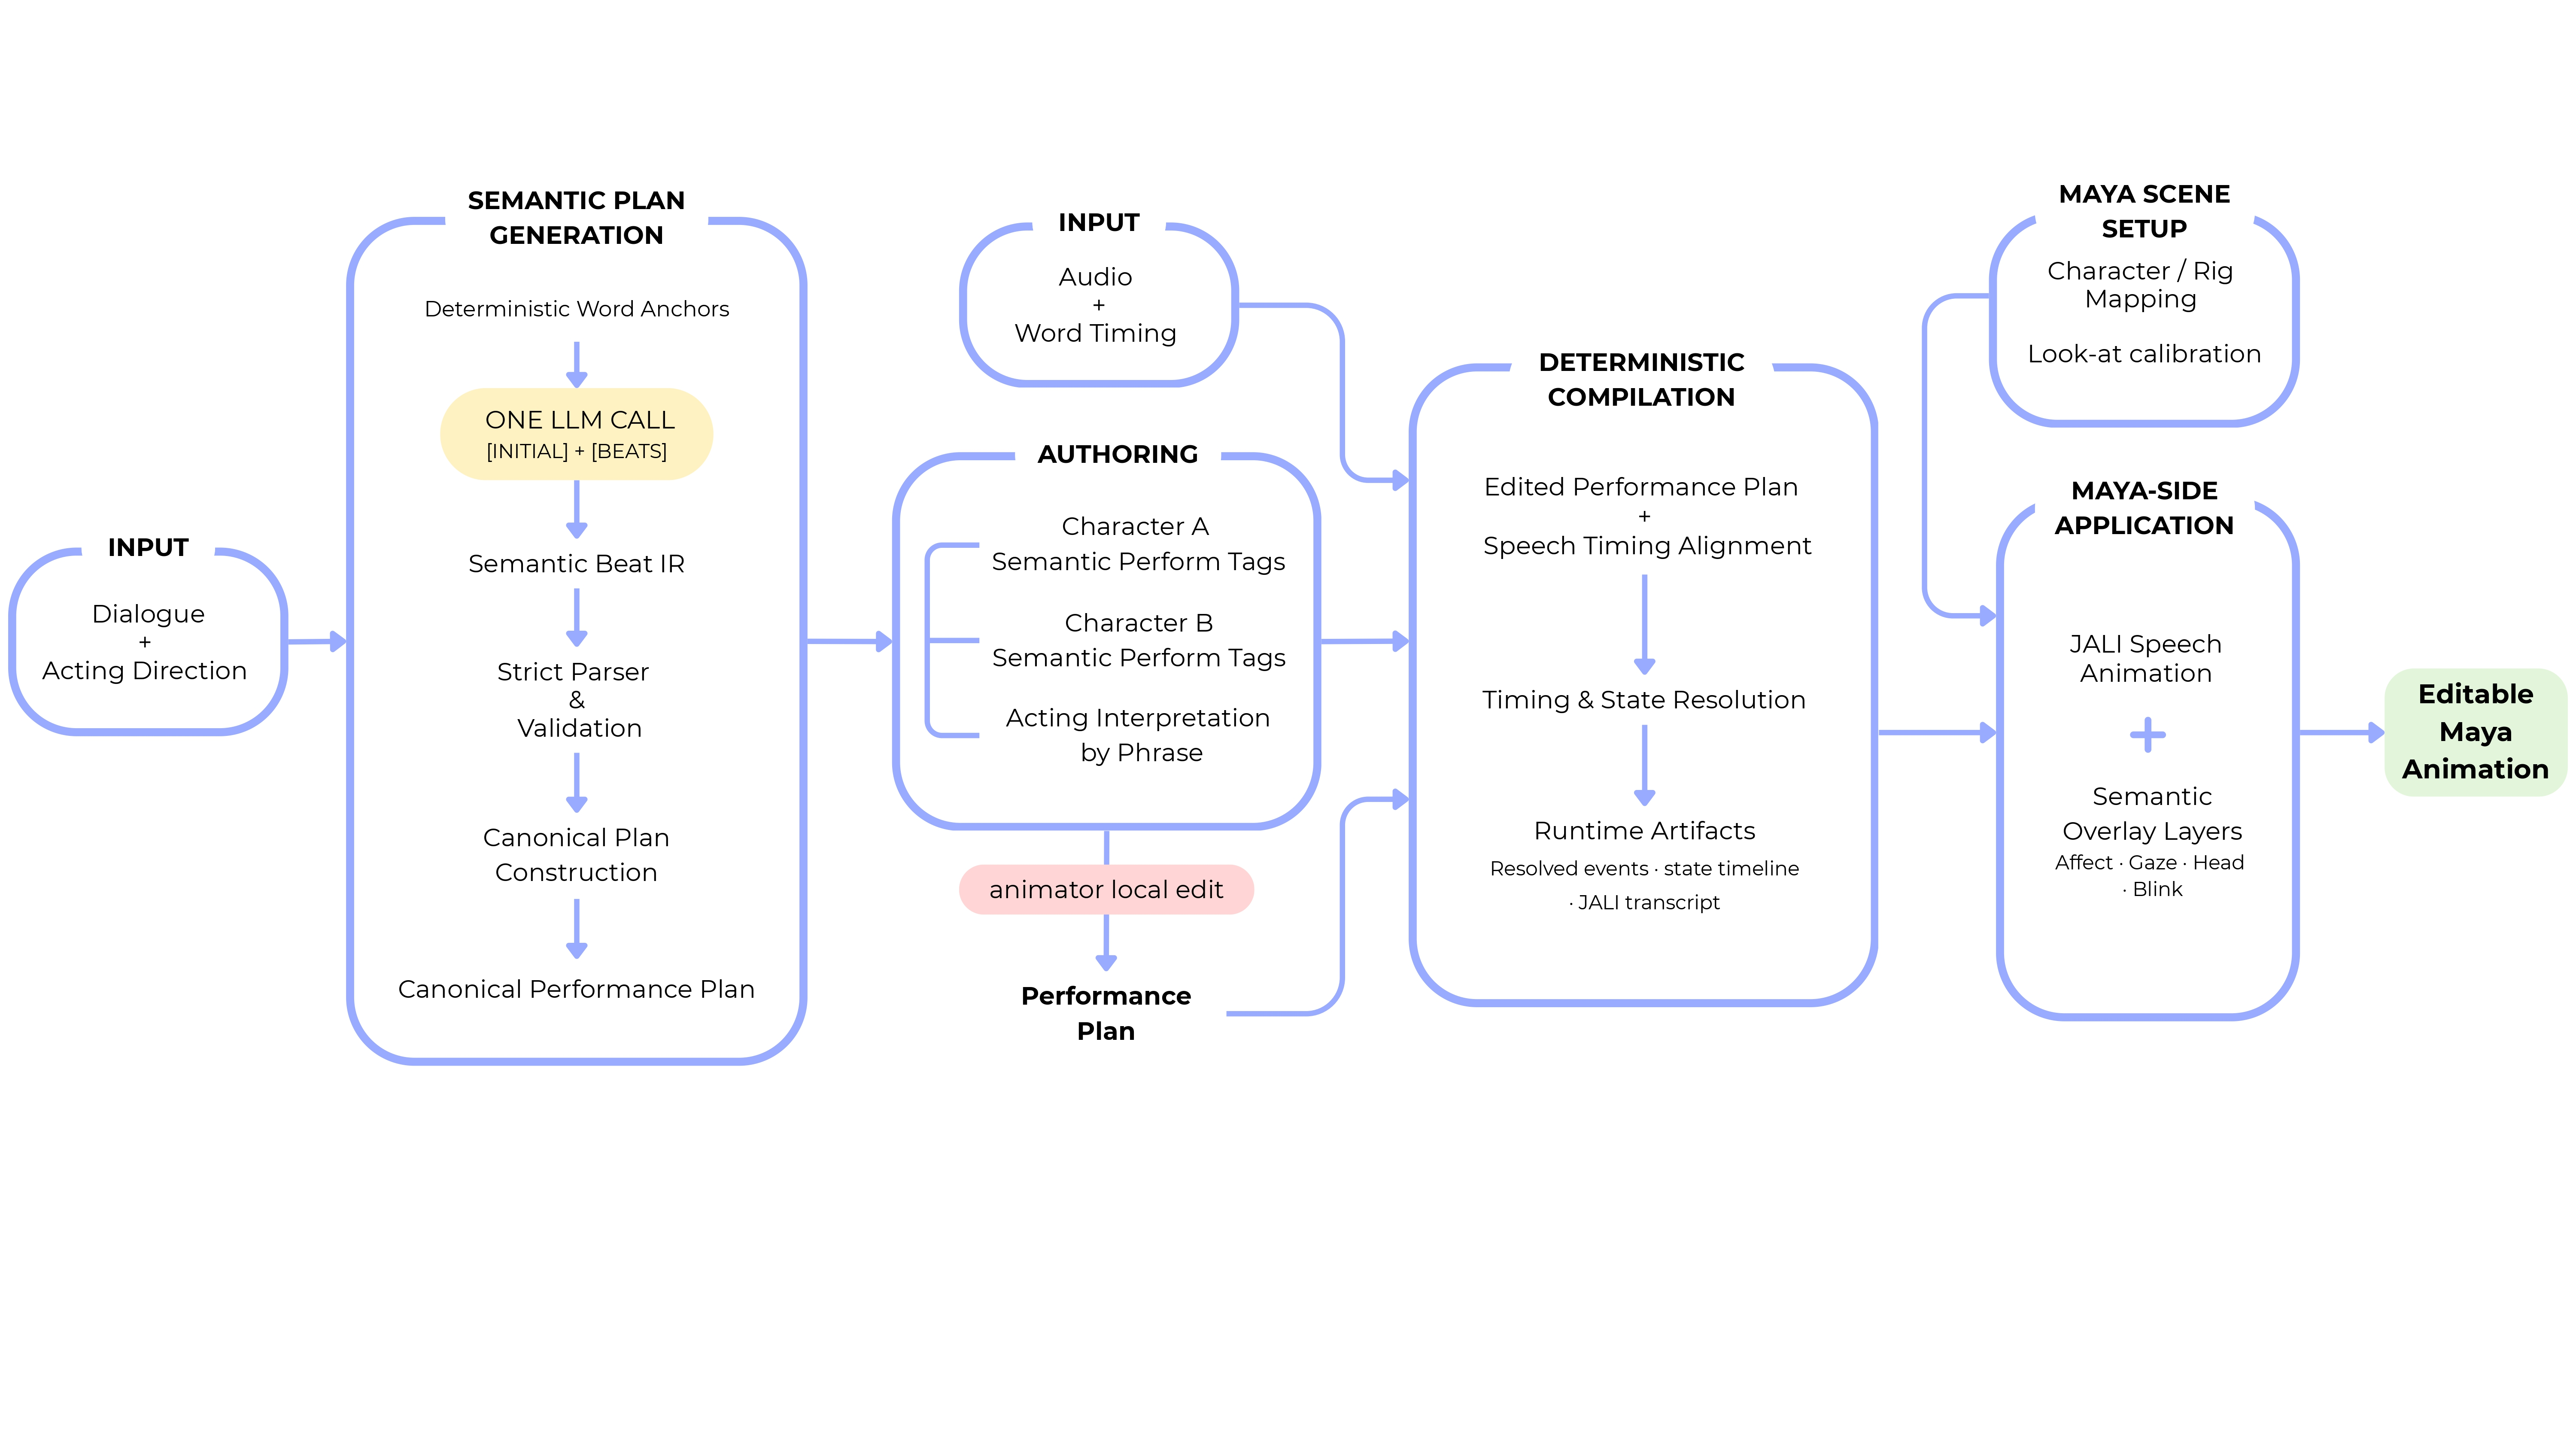
\includegraphics[width=\textwidth]{figures/system_architecture.jpg}
    \caption{System architecture. A single LLM call proposes a shared dyadic semantic interpretation over deterministic dialogue anchors. The canonical backend plan is exposed in Maya as character-specific Semantic Performance Tags; animator edits are resolved and compiled without another LLM call before deterministic JALI and Maya-side application.}
    \Description{A pipeline from dialogue and optional Acting Direction through deterministic word anchors, one LLM call, a validated canonical plan, Semantic Performance Tag authoring, deterministic timing and runtime compilation, and Maya-side speech, affect, gaze, head, and blink application.}
    \label{fig:system-overview}
\end{figure*}

\subsection{Anchored Conversational Context and Performance Interpretation}

The workflow begins with labeled dyadic dialogue, an optional free-text \textit{Acting Direction}, and two explicit character identities. Acting Direction may contain scene information, motivation, relationship context, or performance constraints; identities remain immutable throughout generation.

Before the model call, the system converts dialogue into ordered turns and global word anchors (\texttt{w0001}, \texttt{w0002}, \ldots), each retaining source text, speaker, turn, and position. The LLM selects semantic change points using these stable identifiers, which are reused for editing and timing resolution.

The prototype uses \texttt{gpt-5.6-luna} through the OpenAI API with medium reasoning effort and no task-specific training or fine-tuning. One model call receives immutable dialogue, anchored dialogue with speaker metadata, optional Acting Direction, the character-identity contract, and the executable semantic vocabulary. Output contains an initial state for both characters and sparse semantic beats. Initial states specify visible affect, persistent attention, optional head state, and a concise open-language acting interpretation. Each later beat belongs to one actor, is anchored to a dialogue word, and includes an acting interpretation plus at least one changed executable channel---affect, attention, head, or blink. Acting-only and redundant no-op beats are omitted.

The interpreter considers speaking and listening behavior independently. A listener reaction may be anchored to the earliest semantically sufficient word in the other character's speech rather than delayed to the turn boundary. Attention distinguishes persistent \texttt{focus: TARGET} from a temporary \texttt{eye\_action: brief\_check TARGET}; after validation these become author-facing \texttt{GAZE-*} and \texttt{GLANCE-*} tags, with glances returning to the prior persistent target. Targets may denote either interlocutor, another person, an object/location, or supported directional aversions. Executable affect, head, and blink values use finite supported vocabularies, while \texttt{acting} remains open language.

Model output is parsed and validated before authoring. Unsupported labels, unresolved identities, unknown anchors, malformed attention actions, and duplicate actor/anchor events are rejected rather than guessed. Valid beats compile into \texttt{dual\_performance\_plan\_v2}, which stores ordered identities, per-character initial states, sparse event tracks, semantic gaze-target candidates, and provenance. Redundant persistent no-op changes are removed deterministically while the original generated content remains in provenance.

\subsection{Semantic Performance Tag Authoring}

The Maya interface exposes the canonical plan as a readable projection rather than JSON (Figure~\ref{fig:interface}). In dual mode, each character has a separate Semantic Performance Tag panel over the same immutable dialogue. Dialogue spoken by that panel's character and dialogue heard from the interlocutor are visually distinguished, while tags are rendered separately, making both speaking and listening behavior visible within one conversational timeline. Unlike director-authored transcript tags such as those used by S$^3$ \cite{pan2024s3}, these tags are projected from the model-proposed plan and remain editable before execution.

\begin{figure*}[t]
    \centering
    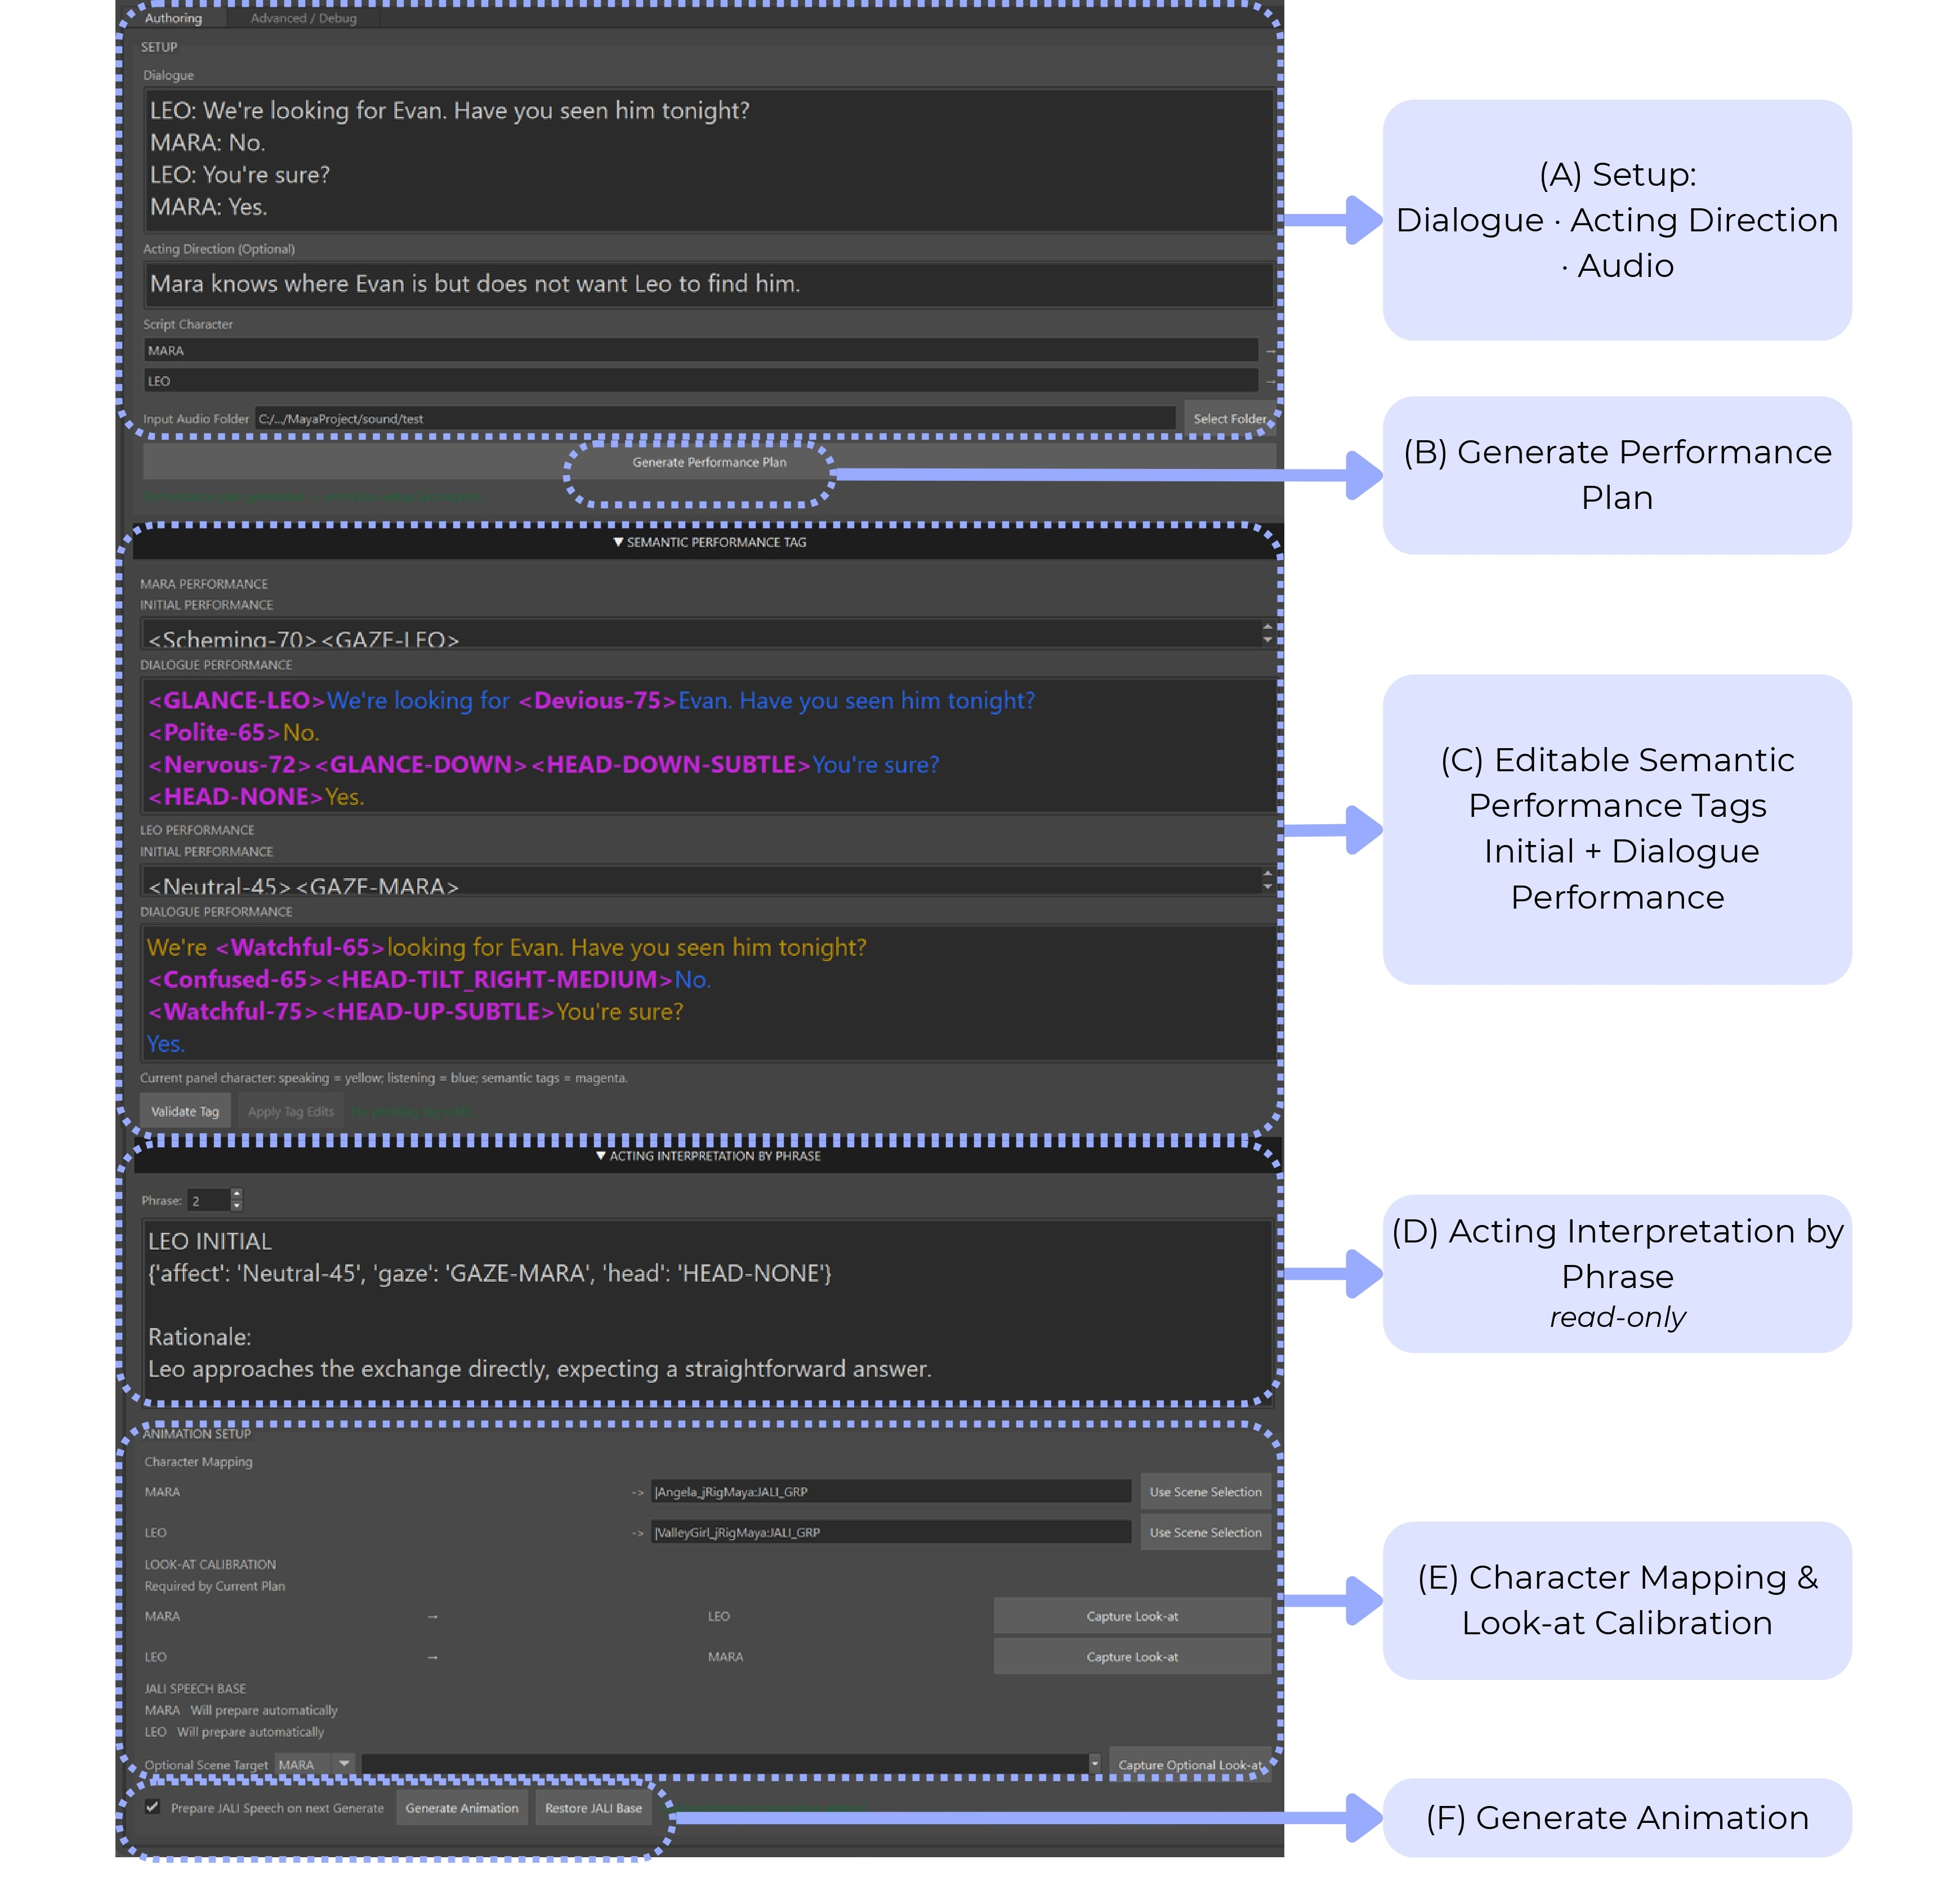
\includegraphics[width=\textwidth]{figures/ui_image.jpg}
    \caption{Participant-facing Maya interface with a filled dyadic example. The interface exposes dialogue and Acting Direction input, generation, editable Semantic Performance Tags for both characters, read-only \textit{Acting Interpretation by Phrase}, character mapping and look-at calibration, and animation generation.}
    \Description{An annotated Maya interface showing a filled dialogue and acting-direction example, the Generate Performance Plan control, two character-specific Semantic Performance Tag editors with initial and dialogue performance, the read-only Acting Interpretation by Phrase section, mapping and calibration, and Generate Animation.}
    \label{fig:interface}
\end{figure*}

Initial persistent state appears before dialogue; later changes appear as compact tags at their anchors. The current editable channels are visible affect, gaze/attention, head behavior, and performative blink. Users may change, add, remove, or reposition valid tag clusters across either character, including several semantic channels in one authoring pass. Dialogue tokens remain immutable, and validation checks the edited projection against the canonical dialogue and executable vocabulary.

Three interface operations separate generation from local editing. \textit{Generate Performance Plan} invokes the backend and loads a validated plan; \textit{Validate Tag} checks local edits without modifying the canonical plan; and \textit{Apply Tag Edits} writes valid edits into the in-memory plan without another LLM call. The original generated acting interpretation associated with each initial state or beat remains visible in a read-only \textit{Acting Interpretation by Phrase} view. When a generated tag is edited, its original interpretation is retained as provenance but marked stale; user-added changes have no original model interpretation.

Rig mappings, audio, and semantic-target-to-Maya look-at calibration remain outside the semantic representation. For each actor--target pair, the animator captures a visually appropriate gaze pose in the current shot. That pose becomes the execution target for a semantic directive such as \texttt{GAZE-B}. The semantic tag therefore does not encode a fixed world-space position or eye rotation. Thus one semantic attention decision can be retained while its visual realization is recalibrated for different cameras, staging, or rigs.

\subsection{Deterministic Compilation to JALI and Maya}

\textit{Generate Animation} treats the edited canonical plan as the source of truth. The LLM does not generate frames, rig coordinates, or animation curves. Instead, the compiler resolves semantic anchors against each character's word-level speech alignment (\texttt{words.jsonl} or a TextGrid \texttt{words} tier). A beat on a character's own word begins at that word's aligned start; a listener beat triggered by the other character begins at the end of the heard word. Persistent affect, gaze, and head state propagate forward, while glances and performative blinks remain event-local.

JALI supplies speech-driven facial animation and executable affect states \cite{edwards2016jali}. For each speaker, the backend constructs an annotated JALI transcript from the resolved affect state over aligned spoken words. Gaze, head, and blink remain in the resolved sparse event representation for deterministic Maya-side application. Persistent focus becomes \texttt{GAZE-*}; a temporary check becomes \texttt{GLANCE-*} and returns to the previously active persistent target. This tagged control abstraction is similar to S$^3$ \cite{pan2024s3}, but here directives are compiled from the edited semantic plan rather than supplied as director-authored transcript input. Character/object targets use calibrated Maya mappings, while directional targets use rig-relative offsets.

\begin{table}[t]
    \centering
    \caption{Mapping from author-facing Semantic Performance Tags to deterministic execution.}
    \label{tab:jiali-mapping}
    \begin{tabular}{p{0.27\columnwidth} p{0.63\columnwidth}}
        \toprule
        \textbf{Semantic field} & \textbf{Deterministic execution} \\
        \midrule
        Acting interpretation &
        Author-facing description; not mapped directly to a rig control. \\

        Affect / intensity &
        Resolved into supported JALI Mask states over aligned speech. \\

        Persistent \texttt{GAZE-*} &
        Maintains the semantic target until a later persistent gaze change. \\

        Temporary \texttt{GLANCE-*} &
        Produces a brief check and returns to the prior target. \\

        Head &
        Compiled to the supported head-control overlay vocabulary. \\

        Blink &
        Compiled to authored eyelid events such as slow/double blinks or eye-close/open holds. \\
        \bottomrule
    \end{tabular}
\end{table}

The compiler writes a dual animation manifest plus resolved per-character events, persistent state timelines, and JALI-annotated transcripts. Maya-side applicators use these artifacts, calibrated look-at poses, and mapped rigs to construct affect, gaze, head, and blink layers. The design boundary is therefore explicit: the LLM proposes \textit{what} the performance means and where semantic changes occur; deterministic code decides \textit{how} those decisions are validated, aligned, and instantiated as animation.

\section{Evaluation}

We used two complementary studies to separate the effect of exposing editable semantic decisions (RQ2--RQ3) from the effect of conversational context on the proposed interpretation itself (RQ1). Study~A compares end-to-end authoring workflows in Maya; Study~B compares text-only Dialogue-Only and Full-Context proposals (Figure~\ref{fig:study-design}).

\begin{figure*}[t]
    \centering
    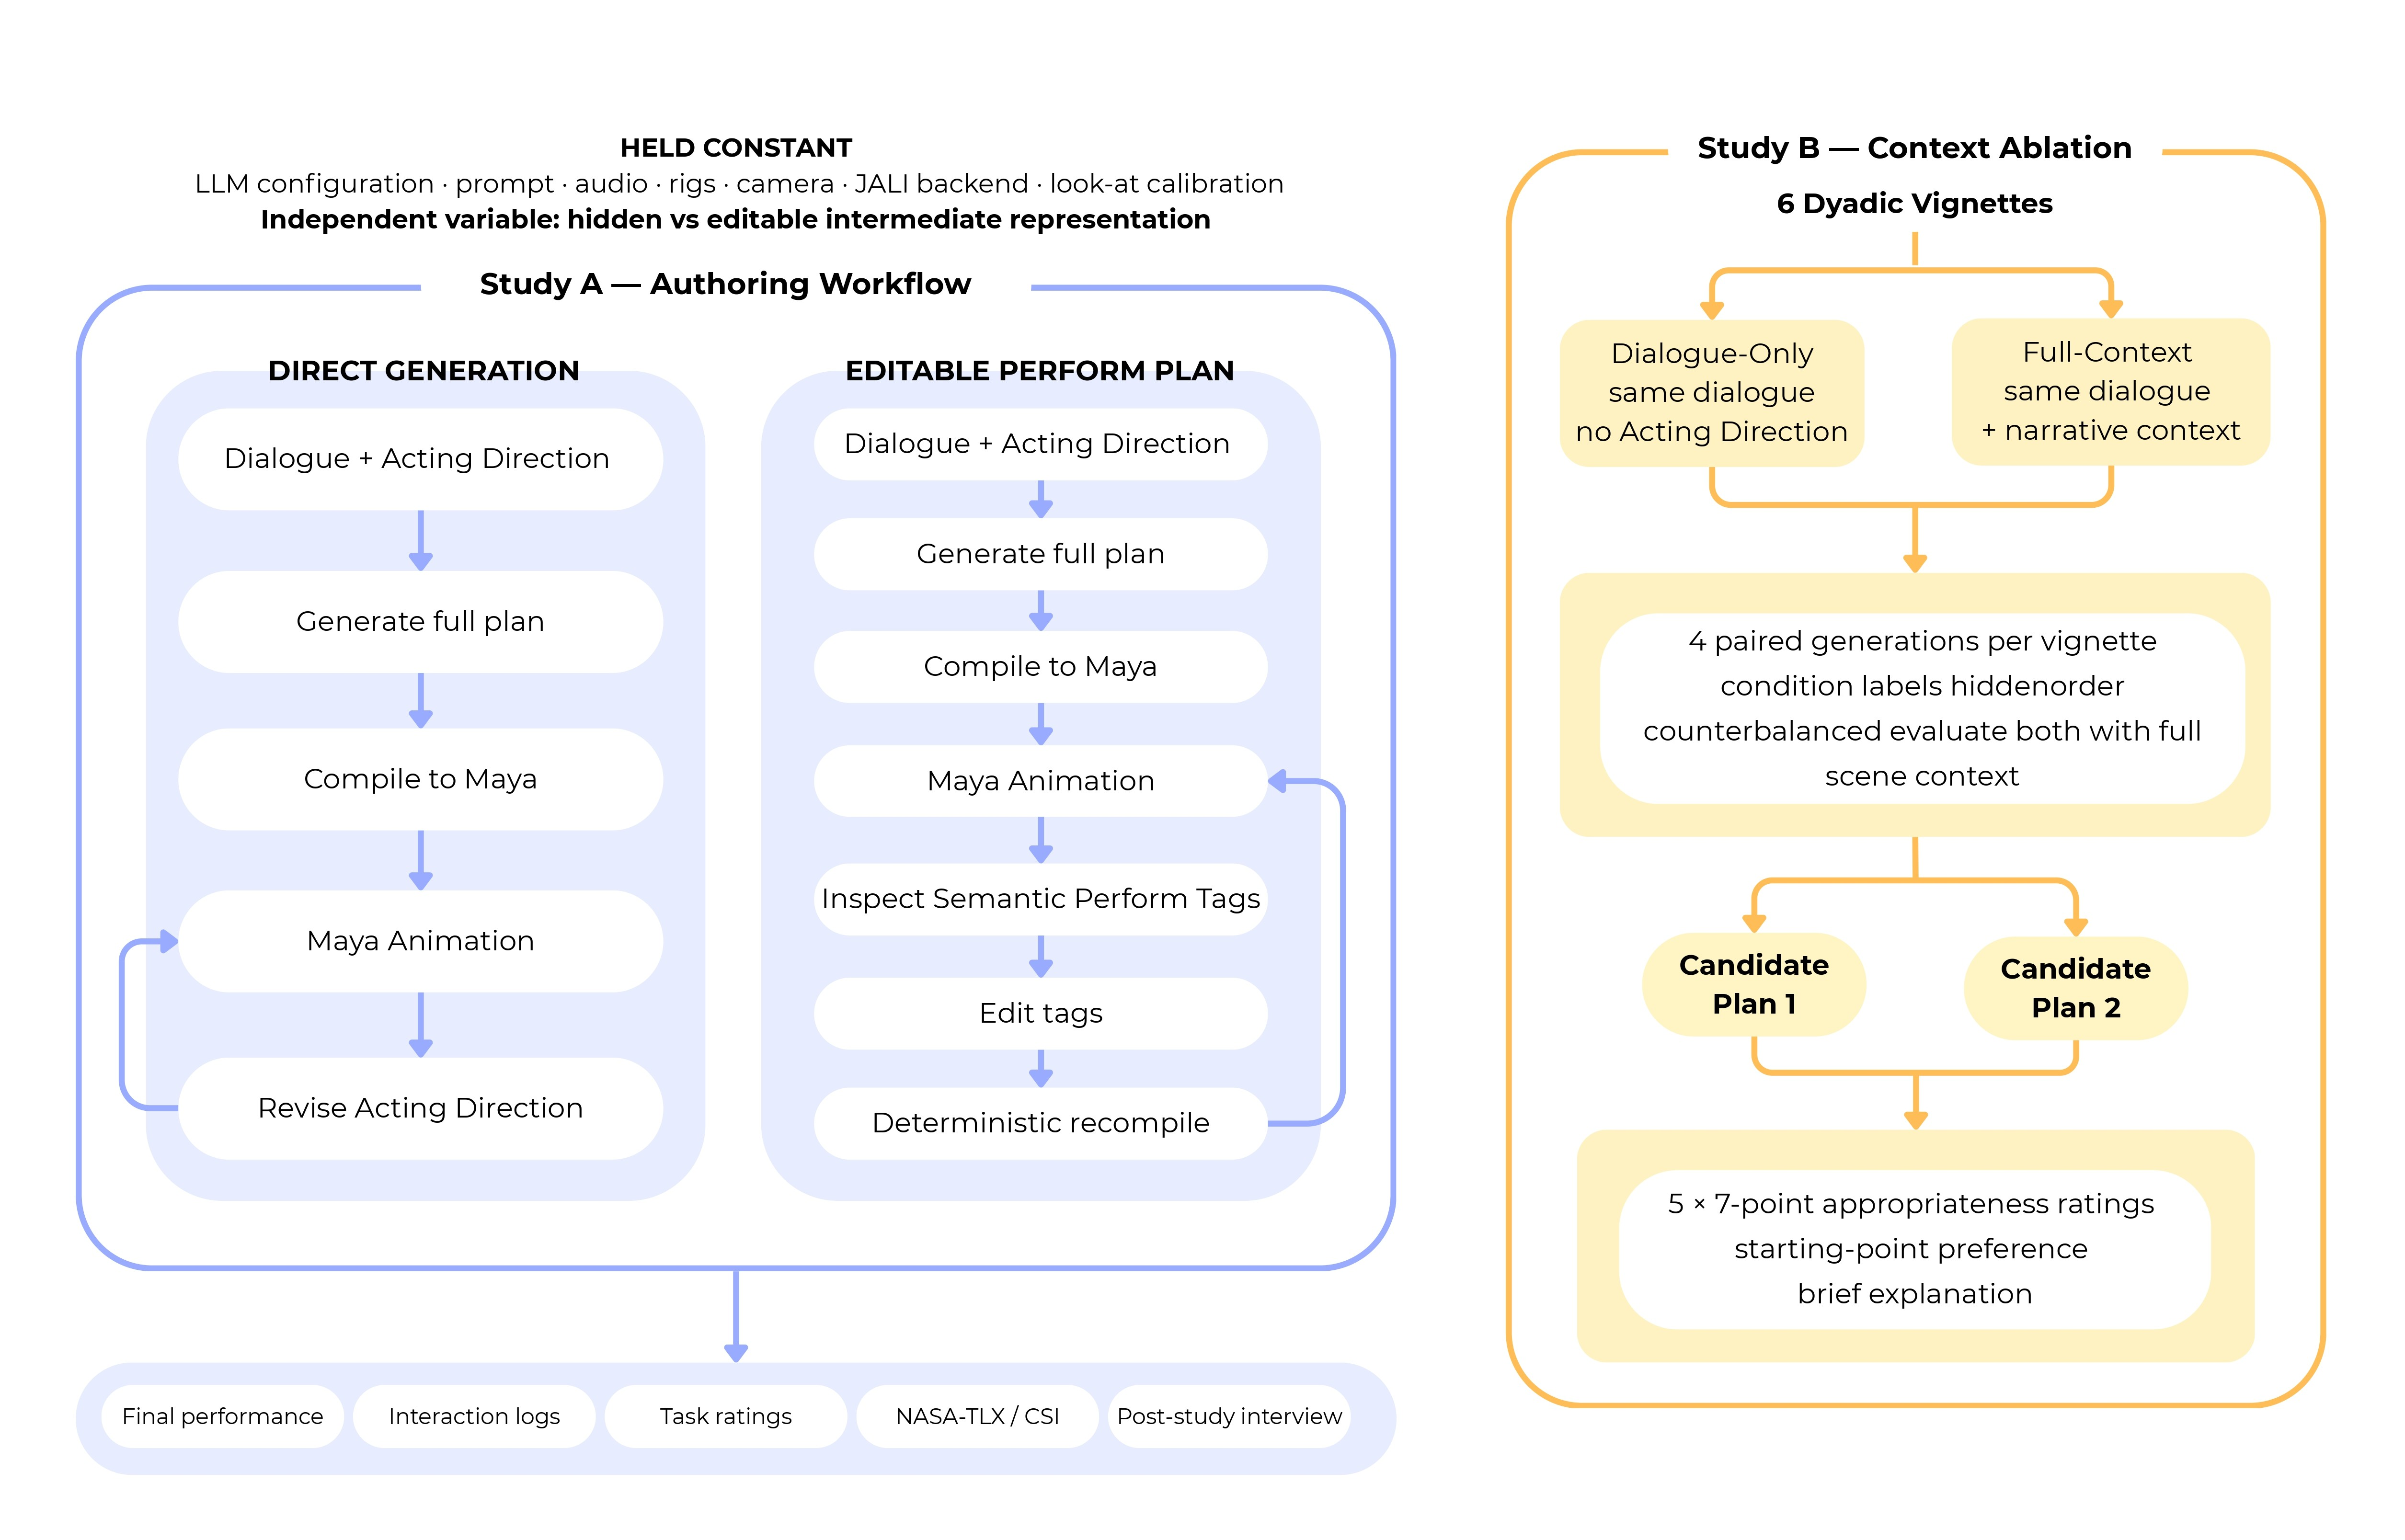
\includegraphics[width=\textwidth]{figures/evaluation_design.jpg}
    \caption{Two-part evaluation. Study~A compares Direct Generation with Editable Semantic Performance Tags in Maya while holding the generation and execution stack constant. Study~B isolates the effect of contextual information on text-only performance proposals across six dyadic vignettes.}
    \Description{Study A is a within-subject comparison between Direct Generation and Editable Semantic Performance Tags. Study B compares Dialogue-Only and Full-Context proposals across six vignettes with condition labels hidden and presentation order counterbalanced.}
    \label{fig:study-design}
\end{figure*}

\subsection{Participants and Overall Procedure}

We analyzed 16 usable participant records. Participants had character-animation or related performance-authoring backgrounds spanning game/film animation, animation/VFX study, professional character animation, and technical animation. Because roles could be selected jointly, eight participants reported game/film animation backgrounds, seven animation/VFX study, three professional animation, and one technical-animation/TD experience. Thirteen reported a numeric duration of relevant experience, spanning 2--15 years ($M=4.69$, $SD=3.54$). Of the 15 participants who completed at least one software-background item, all reported Maya or another keyframe-animation package.

Participants received an explanation of the Semantic Performance Tag fields and completed a short practice example before the formal tasks. The same participants then completed the end-to-end authoring tasks and the text-only context-ablation ratings. Formal stimuli used in Study~A and Study~B did not overlap, and the Study~A tutorial scene was excluded from analysis.

\subsection{Study A: Authoring Workflow Comparison}

\subsubsection{Tasks and Conditions}

Study~A examined whether editable Semantic Performance Tags changed how participants revised system-generated conversational performances. After one tutorial, participants authored both interlocutors in four short dyadic scenes chosen to span complementary context-dependent acting problems such as concealment or suspicion, restrained or affectively incongruent response, evolving interpersonal tension, and relationship repair. Scenes contained exactly two speaking characters and were kept short and comparable in scope. The goal was to make each result match the participant's own reading rather than a reference performance.

The implementation used the same generation and execution path in both conditions; only the visibility and editability of the intermediate semantic representation differed. Both conditions used the same model configuration, dialogue, Acting Direction, scene audio, rigs, cameras, JALI backend, and pre-calibrated semantic look-at targets. Direct low-level Maya curve editing was excluded so that the comparison primarily reflected prompt-level regeneration versus semantic-tag editing.

\paragraph{Direct Generation.}
Participants viewed the generated JALI/Maya animation with the intermediate semantic representation hidden. To revise the acting, they changed the natural-language Acting Direction and regenerated the complete proposal and animation.

\paragraph{Editable Semantic Performance Tags.}
Participants received the same initial dialogue, Acting Direction, model configuration, and generated animation, but could additionally inspect two character-specific tag panels. They could edit affect, persistent or temporary attention, head, and performative-blink decisions across either character. Valid edits updated the existing canonical plan and were deterministically recompiled without another LLM call. The current prototype does not provide field locking or selective LLM regeneration.

Each participant completed two Direct Generation scenes followed by two Editable Semantic Performance Tag scenes. Because workflow order was fixed in the collected sessions, we treat Study~A as a paired first-use comparison and interpret differences with a possible practice/order effect rather than as order-independent causal estimates.

\subsubsection{Interaction Records and Measures}

The prototype retains the original generated canonical plan, edited canonical-plan snapshots where saved, and sidecar session records. These can expose semantic value changes and retained decisions by character and channel (affect, gaze/attention, head, and blink). However, early sessions were not instrumented uniformly enough to support a complete action-by-action reconstruction across all participants. We therefore do not infer population-level accept/modify/remove rates from missing logs; RQ3 is discussed only where saved plan differences directly support the observation.

After each authoring task, participants rated match to intended reading and final satisfaction on seven-point scales. After each two-task workflow block they completed the six raw NASA-TLX dimensions \cite{hart1988nasa} and nine study-specific seven-point workflow items covering expression of acting direction, local revision, revision clarity, final control, dyadic coordination, visual--semantic iteration, creative ownership, alternative exploration, and whether quality justified effort. Items are reported individually rather than as an unvalidated composite. After the editable-tag block, three diagnostic ratings assessed tag-level fit, usefulness of phrase-level interpretation, and the dual-character layout; these were not included in between-workflow tests.

The semi-structured post-study interview focused on the process behind observed edits rather than endorsement of predefined features. It asked how participants judged a performance as complete, what system-proposed decisions they kept, changed, or removed, what they changed first after a mismatch, how prompt regeneration compared with tag editing for alternatives and preservation, where facial channels interacted, whether the dual-character layout aided coordination, when phrase-level interpretations were useful, how semantic gaze targets related to camera/rig decisions, whether the workflow affected authorship or control, and what operations or semantic fields were missing.

\subsubsection{Study A Analysis}

For the two task-level outcomes, we averaged each participant's two tasks within workflow and required two valid task ratings in each workflow. One participant had ambiguous double selections on one Editable-tag task, so the paired task-level tests use $n=15$. The nine workflow items were analyzed item-wise using all valid paired responses ($n=13$--16), and all six NASA-TLX dimensions had $n=16$ paired responses. Given the small sample and ordinal questionnaire outcomes, we use two-sided Wilcoxon signed-rank tests, rank-biserial correlations, and Holm correction within the task-outcome, workflow-item, and NASA-TLX families. Positive rank-biserial values indicate higher Editable-tag ratings; for NASA-TLX, higher values indicate greater workload except performance, where 0 denotes perfect performance and 100 failure.

\subsection{Study B: Context Ablation}

\subsubsection{Stimuli and Conditions}

Study~B isolates semantic interpretation from animation execution and tests whether additional narrative and interpersonal context changes the appropriateness of the proposed performance itself. We constructed six short dyadic vignettes using maximum-variation sampling across contextual dependence and interactional function. Two relatively explicit supportive or confrontational vignettes served as lower-context-dependence cases; four higher-context cases involved concealment, face-saving, tentative affiliation, and relationship repair (Table~\ref{tab:study-b-stimuli}). The vignettes contained no prescriptive facial-animation directions such as named expressions, gaze instructions, head gestures, or blink commands. Context descriptions specified only narrative facts, character relationships, and relevant prior events, leaving performance interpretation to the model.

\begin{table}[t]
    \centering
    \caption{Study~B stimuli vary contextual dependence and interactional function.}
    \label{tab:study-b-stimuli}
    \begin{tabular}{lll}
        \toprule
        \textbf{ID} & \textbf{Context dependence} & \textbf{Interactional problem} \\
        \midrule
        S1 & Low & Explicit support \\
        S2 & Low--moderate & Explicit conflict \\
        S3 & High & Concealment \\
        S4 & High & Face-saving / mixed affect \\
        S5 & High & Tentative affiliation \\
        S6 & High & Relationship repair \\
        \bottomrule
    \end{tabular}
\end{table}

For each vignette we generated shared dyadic proposals under two conditions while holding the model, prompt schema, identities, and decoding configuration constant. Dialogue-Only received labeled dialogue and character identities; Full-Context received the same dialogue plus narrative and interpersonal context through Acting Direction. We generated four independent Dialogue-Only/Full-Context pairs for each vignette, yielding 48 proposals. The replicate pairs were distributed across 16 preconstructed participant packets so that each pair appeared equally often and Dialogue-Only versus Full-Context appeared first equally often across assignments.

The ablation applied only to model input: raters always saw the complete vignette context and dialogue. Each trial showed two anonymized text-only proposals as Plan~A and Plan~B, with hidden condition labels and counterbalanced order; no animation was shown.

\subsubsection{Measures and Analysis}

For each anonymous proposal, participants rated five seven-point criteria (1 = not at all appropriate; 7 = extremely appropriate): overall contextual appropriateness, acting intention, affect, attention/gaze, and dyadic coordination/temporal placement. They then selected Plan~A, Plan~B, or No preference as the preferred animation starting point and could briefly explain the choice.

For each criterion, we averaged the six Dialogue-Only and six Full-Context ratings within participant and compared paired participant-level values with two-sided Wilcoxon signed-rank tests. Overall fit, intention, affect, and gaze use all 16 complete participant pairs; timing uses 15 because one Full-Context timing rating was missing. We report rank-biserial correlations and Holm-adjusted $p$ values across the five criteria. Starting-plan choices are decoded back to condition and reported descriptively across all 96 scene-level questions, retaining No preference, missing, and ambiguous responses separately. Open-ended responses are used only as qualitative context; we make no thematic-frequency claims from questionnaire comments alone.

\section{Discussion}

6.1 Performance as an Editable Interpretation

Generation → interpretation → negotiation → execution.

6.2 Semantic Abstraction for Animation

Performance Plan bridges screenplay semantics and low-level controls.

6.3 Human-AI Agency

AI proposes; animator judges, preserves, contests, revises.

6.4 Explainability

Not model explanation; visibility of creative interpretation.

6.5 Ambiguity as a Feature

No single correct acting choice; support alternatives rather than optimize toward “ground truth.”

6.6 Design Implications

Expose semantic decisions; support partial regeneration; preserve approved choices; connect rationale to evidence.

6.7 Limitations

Small expert sample; JALI dependency; dyadic scope; LLM variability; cultural/acting subjectivity; limited performance channels.
\section{Conclusion}

Narrative context → editable Performance Plan → animator-controlled procedural animation; contribution = making AI performance interpretation an authoring object rather than a hidden generation step.

% ============================================================
% References
% ============================================================
\bibliographystyle{ACM-Reference-Format}
\bibliography{references}

\end{document}
